\documentclass{exam}
%%%%%%%%%%%%%%%%%%%%%%%%%%%%%%%%%%%%%%%%%%%%%%%%%%%%%%%%%%%%%%%%%%%%%%%%%%%%%%%
%  _______  _______  ___      ____   _______
% |       ||       ||   |    |    | |   _   |
% |       ||  _____||   |___  |   | |  |_|  |
% |       || |_____ |    _  | |   | |       |
% |      _||_____  ||   | | | |   | |       |
% |     |_  _____| ||   |_| | |   | |   _   |
% |_______||_______||_______| |___| |__| |__|
%
% Header for CS61A Tutoring TeX Files
%
% Collected and modified by Jonathan Kotker and Thomas Magrino
%
% This package contains references to other packages, new commands, and values
% for different parameters, common to all discussion documents.
% This file should be placed one level above the discussion TeX files in
% the directory tree.
%
% Please modify the appropriate section below with information about
% the class: this information needs to be updated only once per semester.
%%%%%%%%%%%%%%%%%%%%%%%%%%%%%%%%%%%%%%%%%%%%%%%%%%%%%%%%%%%%%%%%%%%%%%%%%%%%%%%

%% Uncomment the following line to display solutions
%\def\discussionsolutions{}

\ProvidesPackage{commonheader}

%%% Packages Needed %%%%%%%%%%%%%%%%%%%%%%%%%%%%%%%%%%%%%%%%%%%%%%%%%%%%%%%%%%%
\usepackage{amsfonts}
\usepackage{amsmath}
\usepackage{bm}
\usepackage{amssymb}
\usepackage{amsthm}
\usepackage{color}
\usepackage{comment}
\usepackage{enumerate}
\usepackage{fancybox}
\usepackage{fix-cm}
\usepackage{float}
\usepackage{fullpage}
\usepackage{graphicx}
\usepackage[pdftex,colorlinks]{hyperref}
\usepackage{import}
\usepackage{listings}
\usepackage{multirow}
\usepackage{multicol}
\usepackage{palatino}
\usepackage{paralist}
\usepackage{parskip}
\usepackage{tabularx}
\usepackage[calcwidth]{titlesec}
\usepackage{upquote}
\usepackage{verbatim}
\usepackage{wasysym}
\usepackage{tikz}
\usepackage{tikz-qtree,tikz-qtree-compat}
\usepackage{synttree}
%%%%%%%%%%%%%%%%%%%%%%%%%%%%%%%%%%%%%%%%%%%%%%%%%%%%%%%%%%%%%%%%%%%%%%%%%%%%%%%

% Define solution style
\unframedsolutions
\renewcommand{\solutiontitle}{}
\SolutionEmphasis{\color{red}}


%%% Information about the class %%%%%%%%%%%%%%%%%%%%%%%%%%%%%%%%%%%%%%%%%%%%%%%
\newcommand{\semester}[1]{\newcommand{\sem}{#1}}
\newcommand{\stafflist}[1]{\newcommand{\staff}{#1}}
%%%%%%%%%%%%%%%%%%%%%%%%%%%%%%%%%%%%%%%%%%%%%%%%%%%%%%%%%%%%%%%%%%%%%%%%%%%%%%%

%%% MODIFY THIS INFORMATION AS NECESSARY %%%%%%%%%%%%%%%%%%%%%%%%%%%%%%%%%%%%%%
\semester{Fall 2022}
\stafflist{Curated by Gene Pan, 
Raman Varma,
Frank Liu,
Nicholas Trong-Nhan Nguyen,
Elisa Kim,
Riya Singhal,
Ryan Campbell,
Issac Chen,
Vy Ho,
Jaewon Dong, and 
Jonathan Chen in association with Gabe Classon, 
Aditya Balasubramanian, and
Maya Romero
}
%%%%%%%%%%%%%%%%%%%%%%%%%%%%%%%%%%%%%%%%%%%%%%%%%%%%%%%%%%%%%%%%%%%%%%%%%%%%%%%

%%% Margins and definitions %%%%%%%%%%%%%%%%%%%%%%%%%%%%%%%%%%%%%%%%%%%%%%%%%%%
\setlength{\marginparwidth}{1.2in}
\let\oldmarginpar\marginpar
\renewcommand{\marginpar}[1]{\-\oldmarginpar[\raggedleft\footnotesize #1]%
{\raggedright\footnotesize #1}}
%%%%%%%%%%%%%%%%%%%%%%%%%%%%%%%%%%%%%%%%%%%%%%%%%%%%%%%%%%%%%%%%%%%%%%%%%%%%%%%

%%% Configuring the document title %%%%%%%%%%%%%%%%%%%%%%%%%%%%%%%%%%%%%%%%%%%%
\definecolor{titlecol}{gray}{0.6}

% \titlebreak is used to insert a break in the title of the page without 
% causing a break in the running footer. 
\newcommand{\titlebreak}{\par}

\let\oldtitle\title
\renewcommand{\title}[1]
    {\oldtitle{
      
        {\begin{flushright}
            \huge {\sc{#1}}
            \fontsize{45}{0} \sffamily \color{titlecol} \selectfont
            \ifdefined\discussionmetas
              \marginpar{\Large{\textcolor{blue}{Meta}}}
            \else
              \ifdefined\discussionsolutions
                \marginpar{\Large{\textcolor{red}{Solutions}}}
              \fi
            \fi
        \end{flushright}}
        \rule{\textwidth}{0.2em}}
    \newcommand{\disctitle}{#1}}
%%%%%%%%%%%%%%%%%%%%%%%%%%%%%%%%%%%%%%%%%%%%%%%%%%%%%%%%%%%%%%%%%%%%%%%%%%%%%%%

%%% Configuring the header and footer %%%%%%%%%%%%%%%%%%%%%%%%%%%%%%%%%%%%%%%%%
\newcommand{\discnumber}[1]{\newcommand{\discnum}{#1}}

\pagestyle{headandfoot}
\firstpagefootrule
\firstpagefooter{\small \staff}{}{}
\runningfootrule
\runningfooter{
  \let\titlebreak\relax
  \sc \oddeven{Midterm 2 Review Session}{\thepage}}{}{\sc \oddeven{\thepage}{CSM 61A \sem}
  }

\let\oldmaketitle\maketitle
\renewcommand{\maketitle}[0]{\oldmaketitle \thispagestyle{headandfoot}}

%%%%%%%%%%%%%%%%%%%%%%%%%%%%%%%%%%%%%%%%%%%%%%%%%%%%%%%%%%%%%%%%%%%%%%%%%%%%%%%

%%% Configuring the section and subsection titles %%%%%%%%%%%%%%%%%%%%%%%%%%%%%
\titleformat{\section}[hang]{\sffamily \bfseries}
{\fontsize{15}{25} \color{titlecol} \selectfont \thesection}{10pt}
{\fontfamily{ppl} \fontsize{15}{0} \selectfont \raggedleft}
[{\titlerule[1.0pt]}]

\titleformat{\subsection}[hang]{\sffamily \bfseries}
{\thesubsection}{10pt}{}[{\titlerule[0.5pt]}]
%%%%%%%%%%%%%%%%%%%%%%%%%%%%%%%%%%%%%%%%%%%%%%%%%%%%%%%%%%%%%%%%%%%%%%%%%%%%%%%

%%% Colored titles for sections %%%%%%%%%%%%%%%%%%%%%%%%%%%%%%%%%%%%%%%%%%%%%%%
\newcommand{\colorsec}[2]{\section[#1]{{\color{#2} #1}}}
\newcommand{\colorsubsec}[2]{\subsection[#1]{{\color{#2} #1}}}
\newcommand{\colorsubsubsec}[2]{\subsubsection[#1]{{\color{#2} #1}}}
%%%%%%%%%%%%%%%%%%%%%%%%%%%%%%%%%%%%%%%%%%%%%%%%%%%%%%%%%%%%%%%%%%%%%%%%%%%%%%%

%%% Commands used to add rules to tables and figures %%%%%%%%%%%%%%%%%%%%%%%%%%
\floatstyle{ruled}
\newfloat{ruledfigure}{tbph!}{lop}
\floatname{ruledfigure}{Figure}

\newfloat{ruledtable}{tbph!}{lop}
\floatname{ruledtable}{Table}
%%%%%%%%%%%%%%%%%%%%%%%%%%%%%%%%%%%%%%%%%%%%%%%%%%%%%%%%%%%%%%%%%%%%%%%%%%%%%%%

%%% Commands for references %%%%%%%%%%%%%%%%%%%%%%%%%%%%%%%%%%%%%%%%%%%%%%%%%%%
\renewcommand{\eqref}[1]{\hyperref[#1]{Equation \ref*{#1}}}
\newcommand{\exref}[1]{\hyperref[#1]{exercise \ref*{#1}}}
\newcommand{\figref}[1]{\hyperref[#1]{Figure \ref*{#1}}}
\newcommand{\lccderef}[1]{\hyperref[#1]{LCCDE \ref*{#1}}}
\newcommand{\quesref}[1]{\hyperref[#1]{question \ref*{#1}}}
\newcommand{\secref}[1]{\hyperref[#1]{section \ref*{#1}}}
\newcommand{\stepref}[1]{\hyperref[#1]{step \ref*{#1}}}
\newcommand{\tableref}[1]{\hyperref[#1]{Table \ref*{#1}}}
\renewcommand{\equationautorefname}{equation}
%%%%%%%%%%%%%%%%%%%%%%%%%%%%%%%%%%%%%%%%%%%%%%%%%%%%%%%%%%%%%%%%%%%%%%%%%%%%%%%

%%% Useful new commands %%%%%%%%%%%%%%%%%%%%%%%%%%%%%%%%%%%%%%%%%%%%%%%%%%%%%%%
\newcommand{\email}[1]{\href{#1}{{\tt #1}}}

\newcommand{\super}[1]{\ensuremath{^{\textrm{#1}}}}
\newcommand{\sub}[1]{\ensuremath{_{\textrm{#1}}}}

\newcommand{\boxtext}[2]{\framebox{\parbox[b]{#1}{#2}}}

% Defining terms
\newcommand{\define}[1]{\textbf{#1}}

% Rendering an unnumbered footnote
\makeatletter
\long\def\unmarkedfootnote#1{{\long\def\@makefntext##1{##1}\footnotetext{#1}}}
\makeatother
%%%%%%%%%%%%%%%%%%%%%%%%%%%%%%%%%%%%%%%%%%%%%%%%%%%%%%%%%%%%%%%%%%%%%%%%%%%%%%%

%%% Box sizes %%%%%%%%%%%%%%%%%%%%%%%%%%%%%%%%%%%%%%%%%%%%%%%%%%%%%%%%%%%%%%%%%
%%% These parameters determine the sizes of the boxes used %%%%%%%%%%%%%%%%%%%%
%%% to explain special and/or subtle points. %%%%%%%%%%%%%%%%%%%%%%%%%%%%%%%%%%
%%%%%%%%%%%%%%%%%%%%%%%%%%%%%%%%%%%%%%%%%%%%%%%%%%%%%%%%%%%%%%%%%%%%%%%%%%%%%%%
\newcommand{\boxlarge}{6.40in}
\newcommand{\boxmed}{6.05in}
\newcommand{\boxsmall}{5.75in}
%%%%%%%%%%%%%%%%%%%%%%%%%%%%%%%%%%%%%%%%%%%%%%%%%%%%%%%%%%%%%%%%%%%%%%%%%%%%%%%

%%% Miscellaneous parameters %%%%%%%%%%%%%%%%%%%%%%%%%%%%%%%%%%%%%%%%%%%%%%%%%%
\setlength{\parindent}{0in}
%\settimeformat{ampmtime}
\allowdisplaybreaks
%%%%%%%%%%%%%%%%%%%%%%%%%%%%%%%%%%%%%%%%%%%%%%%%%%%%%%%%%%%%%%%%%%%%%%%%%%%%%%%

%%% Mathematical commands %%%%%%%%%%%%%%%%%%%%%%%%%%%%%%%%%%%%%%%%%%%%%%%%%%%%%
\newcommand{\surjects}{\twoheadrightarrow}
\newcommand{\injects}{\hookrightarrow}
\newcommand{\isom}{\simeq}
\newcommand{\notdiv}{\nmid}
\newcommand{\del}{\partial}
\newcommand{\Intersection}{\bigcap} % intersection of a collection
\newcommand{\intersect}{\cap} % binary intersection
\newcommand{\Union}{\bigcup} % union of a collection
\newcommand{\union}{\cup} % binary union
\newcommand{\tensor}{\otimes}
\newcommand{\directsum}{\oplus} % binary direct sum
\newcommand{\Directsum}{\bigoplus} % direct sum of a collection
\newcommand{\isomto}{\overset{\sim}{\rightarrow}}

% Expected value
\newcommand{\E}[0]{\ensuremath{\mathbb{E}}}

% Probability (of an event)
\renewcommand{\P}[0]{\ensuremath{\mathbb{P}}}

% Variance/covariance
\newcommand{\var}[0]{\text{var}}
\newcommand{\cov}[0]{\text{cov}}

% Fraction w/parens around it
\newcommand{\pfrac}[2]{\ensuremath{\left(\frac{#1}{#2}\right)}}

% Fraction you can use even if you're not in math mode
\newcommand{\mfrac}[2]{\ensuremath{\frac{#1}{#2}}}

% "maybe equal" - equal with a ? sign on top
\newcommand{\meq}[0]{\ensuremath{\stackrel{?}{=}}}

% maybe anything - anything with a ? on top
\newcommand{\maybe}[1]{\ensuremath{\stackrel{?}{#1}}}

% \problem{1.1} gives you a spiffy-looking "Problem 1.1"
\newcommand{\problem}[1]{ \vspace{.15in} \noindent{\bf Problem #1} \quad\\
\noindent}

% negative/positive infinity
\newcommand{\ninfty}[0]{{\ensuremath{{-\infty}}}}
\newcommand{\pinfty}[0]{{\ensuremath{{+\infty}}}}

% Derivative wrt argument
\newcommand{\der}[1]{\ensuremath{\frac{d}{d #1}}}

% Partial derivative of arg1 wrt arg2
\newcommand{\pder}[2]{\ensuremath{\frac{\partial #1}{\partial #2}}}

% nth derivative
\newcommand{\nder}[2]{\ensuremath{\frac{d^{#2}}{d #1^{#2}}}}

% floor and ceiling
\newcommand{\floor}[1]{\ensuremath{\lfloor{} #1 \rfloor{}}}
\newcommand{\ceil}[1]{\ensuremath{\lceil{} #1 \rceil{}}}

% like \boxed{} but for text instead of math
\newcommand{\tboxed}[1]{\boxed{\text{#1}}}

% creates a \tboxed{} with an invisible charater
\newcommand{\tphan}[1]{\tboxed{\phantom{#1}}}

\def\({\left(}
\def\){\right)}

\def\<{\left\langle}
\def\>{\right\rangle}

% For lemmas
\newtheorem{lemma}{Lemma}

% For Python code
\lstset{language=Python,
        basicstyle=\ttfamily,
        commentstyle=\ttfamily,
        showstringspaces=false,
        breaklines=true,
        breakatwhitespace=true,
}

% For Scheme code
\lstdefinelanguage{Scheme}{
  morekeywords=[1]{define, define-syntax, define-macro, lambda, define-stream,
                   stream-lambda},
  morekeywords=[2]{begin, call-with-current-continuation, call/cc,
                   call-with-input-file, call-with-output-file, case, cond, do,
                   else, for-each, if, let*, let, let-syntax, letrec,
                   letrec-syntax, let-values, let*-values, and, or, not, delay,
                   force, quasiquote, quote, unquote, unquote-splicing, map,
                   fold, syntax, syntax-rules, eval, environment, query},
  morekeywords=[3]{import, export},
  alsodigit=!\$\%&*+-./:<=>?@^_~,
  sensitive=true,
  morecomment=[l]{;},
  morecomment=[s]{\#|}{|\#},
  morestring=[b]",
  basicstyle=\ttfamily,
  keywordstyle=\bf\ttfamily,
  upquote=true,
  breaklines=true,
  breakatwhitespace=true,
  literate=*{`}{{`}}{1}
}

% Creates a minipage environment, which can be used to section off text so that
% it won't be split between two pages. Minipage sets the parskip variable to 0,
% so this preserves the value in the minipage environment.
%
% Source:
% http://tex.stackexchange.com/questions/43002/how-to-preserve-the-same-parskip-in-minipage
\newlength{\currentparskip}
\newenvironment{blocksection}
{
    \setlength{\currentparskip}{\parskip}% save the value
    \begin{minipage}{\linewidth}
    \setlength{\parskip}{\currentparskip}% restore the value
}
{
    \end{minipage}
}

%%%%%%%%%%%%%%%%%%%%%%%%%%%%%%%%%%%%%%%%%%%%%%%%%%%%%%%%%%%%%%%%%%%%%%%%%%%%%%%

% Use \printanswers to print with answers and \noprintanswers to print without.
% Check for defined flag \discussionsolutions to show solutions
\ifdefined\discussionsolutions
  \printanswers
\else
  \noprintanswers
\fi

% Meta information is mentor-facing information to assist with teaching the 
% worksheet. Information is presented in blue. 

\ifdefined\discussionmetas
    \newenvironment{meta}{\color{blue}}{}
    \newenvironment{questionmeta}{
      \begin{solution}
      \color{blue}
    }{
      \end{solution}
    }
\else
    \newenvironment{meta}{\comment}{\endcomment}
    \newenvironment{questionmeta}{\comment}{\endcomment}
\fi

% Backward compatibility with old templates that use "guide"
\let\guide\meta

% The nonsol environment will show items within it only if answers are not set
% to be printed. Useful for hiding docstring in worksheet solutions.
\newenvironment{nonsol}{}{}
\ifdefined\discussionsolutions
    \excludecomment{nonsol}
\else
\fi
%%%%%%%%%%%%%%%%%%%%%%%%%%%%%%%%%%%%%%%%%%%%%%%%%%%%%%%%%%%%%%%%%%%%%%%%%%%%%%%

\author{ \Large \sc Computer Science Mentors 61A}

\usepackage{outlines}

%%% CHANGE THESE %%%%%%%%%%%%%%%%%%%%%%%%%%%%%%%%%%%%%%%%%%%%%%%%%%%%%%%%%%%%%%
\discnumber{9}
\title{\textsc{Midterm 2 Review Session}}
\date{October 23, 2022}
%%%%%%%%%%%%%%%%%%%%%%%%%%%%%%%%%%%%%%%%%%%%%%%%%%%%%%%%%%%%%%%%%%%%%%%%%%%%%%%

\begin{document}
    \maketitle
    \rule{\textwidth}{0.15em}
%    \fontsize{12}{15}\selectfont


\section{Recursion}
\begin{questions}
\begin{blocksection}
\question \textbf{Skipping Around} (Su21 MT2 Q2b)

A skip list is defined as a sublist of a list such that each element in the sublist is non adjacent in the
original list. For original list \lstinline{[5, 6, 8, 2]}, the lists \lstinline{[5, 8]}, \lstinline{[5, 2]}, \lstinline{[6, 2]}, \lstinline{[5]}, \lstinline{[6]}, \lstinline{[8]}, \lstinline{[2]}, \lstinline{[]} are
all skip lists of the original list. The empty list is always a skip list of any list.

Given a list \lstinline{int_lst} of unique integers, return a list of all unique skip lists of \lstinline{int_lst} where each skip
list contains integers in strictly increasing order. The order in which the skip lists are returned does not matter.
    
\begin{lstlisting}
def list_skipper(int_list):
    """
    >>> list_skipper([5,6,8,2])
    [[5, 8], [5], [6], [8], [2], []]
    >>> list_skipper([1,2,3,4,5])
    [[1, 3, 5], [1, 3], [1, 4], [1, 5], [1], [2, 4], [2, 5], [2], [3, 5], [3], [4], [5], []]
    >>> list_skipper([])
    [[]]
    """
    if len(int_lst) == 0:

        return _____________________________

    with_first = _____________________________

    without_first = _____________________________

    with_first = [ _________ for x in with_first if x == [] 
    
        or ____________]

    return with_first + without_first
\end{lstlisting}
\end{blocksection}
\begin{solution}
    \begin{lstlisting}
    def list_skipper(int_list):
        if len(int_lst) == 0:
            return [[]]
        with_first = list_skipper(int_lst[2:])
        without_first = list_skipper(int_lst[1:])
        with_first = [ [int_lst[0]] + x for x in with_first if x == [] or x[0] > int_lst[0]]
        return with_first + without_first
    \end{lstlisting}
\end{solution}
\begin{blocksection}
\question \textbf{maxkd} (Su20 MT1 Q3)

\begin{lstlisting}
def maxkd(meteor, k):
    """
    Given a number `meteor`, finds the largest number of length `k` or fewer,
    composed of digits from `meteor`, in order.

    >>> maxkd(1234, 1)
    4
    >>> maxkd(32749, 2)
    79
    >>> maxkd(1917, 2)
    97
    >>> maxkd(32749, 18)
    32749
    """
    if ______________________________________:

        return ______________________________________

    a = ______________________________________

    b = ______________________________________

    return ______________________________________
\end{lstlisting}
\end{blocksection}
\begin{solution}
    \begin{lstlisting}
def maxkd(meteor, k):
    """
    Given a number `meteor`, finds the largest number of length `k` or fewer,
    composed of digits from `meteor`, in order.

    >>> maxkd(1234, 1)
    4
    >>> maxkd(32749, 2)
    79
    >>> maxkd(1917, 2)
    97
    >>> maxkd(32749, 18)
    32749
    """
    if meteor == 0 or k == 0:
        return 0
    a = maxkd(meteor // 10, k - 1) * 10 + meteor % 10
    b = maxkd(meteor // 10, k)
    return max(a, b)
\end{lstlisting}
\end{solution}

\end{questions}

\section{Lists, Mutability, and Dictionaries}

\begin{questions}
\begin{blocksection}
\question \textbf{Protect the Environment} (Fa19 Final Q2)

Draw the environment diagram that results from running the following code.
\begin{lstlisting}
def cold(d):
    day = rain[:1]
    night = lambda: len(day)
    cold = rain.pop()
    day = d
    return night
rain = [3, 4]
d, day = [5], [lambda: d]
cold(rain + [day[0](), rain])()
\end{lstlisting}
\begin{solution}[5in]
    \url{https://tinyurl.com/ms67cb5c}

    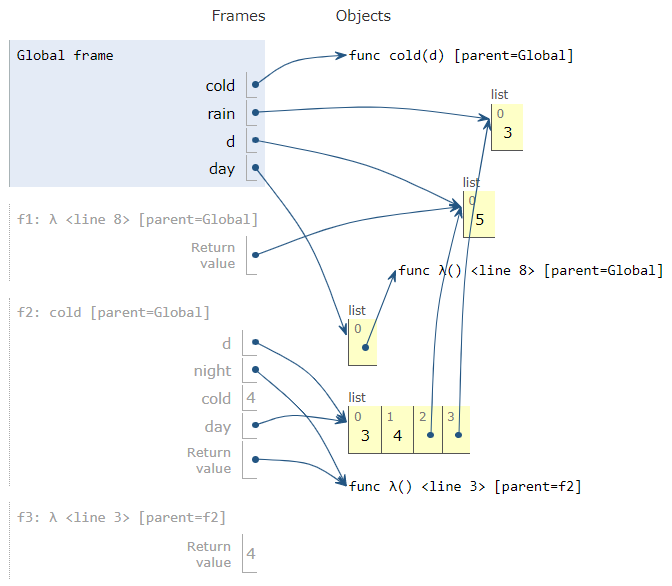
\includegraphics[width=0.8\textwidth]{protecttheenvironment.png}
\end{solution}
\end{blocksection}

\begin{blocksection}
\question \textbf{Wait 'til You See What's in Store} (Su21 MT Q5a)

Implement \lstinline{memory_store}, a function that will return two functions: \lstinline{add_val} and \lstinline{times_seen}. When called on a number \lstinline{var1}, \lstinline{times_seen} will return the number of times \lstinline{add_val} has been called on that particular value \lstinline{var1}.

\begin{lstlisting}
def memory_store():
    """
    >>> add_val, times_seen = memory_store()
    >>> add_val(4)
    >>> for _ in range(3):
    ... add_val(3)
    >>> times_seen(3)
    3
    >>> times_seen(4)
    1
    >>> times_seen(2)
    0
    >>> add_val(3)
    >>> times_seen(3)
    4
    """
    memory = {}
    def add_val(var1):
        if var1 in memory:

            ______________________________________
        else:

            ______________________________________

    def times_seen(var1):

        return ______________________________________
    return add_val, times_seen
\end{lstlisting}
\end{blocksection}
\begin{solution}
\begin{lstlisting}
def memory_store():
    """
    >>> add_val, times_seen = memory_store()
    >>> add_val(4)
    >>> for _ in range(3):
    ... add_val(3)
    >>> times_seen(3)
    3
    >>> times_seen(4)
    1
    >>> times_seen(2)
    0
    >>> add_val(3)
    >>> times_seen(3)
    4
    """
    memory = {}
    def add_val(var1):
        if var1 in memory:
            memory[var1] = memory[var1] + 1
        else:
            memory[var1] = 1
    def times_seen(var1):
        return memory.get(var1, 0)
    return add_val, times_seen
    \end{lstlisting}
\end{solution}
\end{questions}

\newpage
\section{Efficiency}
\begin{questions}
\begin{blocksection}
\question What is the runtime of the following function?
\begin{lstlisting}
def mystery(n):
    for i in range(10000):
        print(n)
\end{lstlisting}

\begin{solution}[1in]
Constant, because we run 10,000 operations no matter the size of \lstinline{n}
\end{solution}
\end{blocksection}

\begin{blocksection}
\question What is the runtime of the following function?
\begin{lstlisting}
def mystery(n):
    a = 0
    for i in range(n):
        for j in range(i, n):
            a += 1
\end{lstlisting}

\begin{solution}[1in]
Quadratic because we are doing $\sim n\cdot n$ operations.
\end{solution}
\end{blocksection}

\begin{blocksection}
    \question What is the runtime of the following function?
    \begin{lstlisting}
def mystery(n):
    i = 1
    while n:
        i = i * 3
        n = n // 3
    return i
    \end{lstlisting}
    
\begin{solution}[1in]
Logarithmic because $n$ must triple to increase the number of operations by 1. 
\end{solution}
\end{blocksection}

\end{questions}

\section{Iterators and Generators}

\begin{questions}
    
\begin{blocksection}
\question \textbf{Yield Fibonacci!} (Fa20 MT2 Q2a)

    Implement \lstinline{fibs}, a generator function that takes a one-argument pure function \lstinline{f} and yields all Fibonacci numbers \lstinline{x} for which \lstinline{f(x)} returns a true value.
    
    The Fibonacci numbers begin with \lstinline{0} and then \lstinline{1}. Each subsequent Fibonacci number is the sum of the previous two. Yield the Fibonacci numbers in order.
\begin{lstlisting}
def fibs(f):
    """Yield all Fibonacci numbers x for which f(x) is a true value.
    >>> odds = fibs(lambda x: x % 2 == 1)
    >>> [next(odds) for i in range(10)]
    [1, 1, 3, 5, 13, 21, 55, 89, 233, 377]
    >>> bigs = fibs(lambda x: x > 20)
    >>> [next(bigs) for i in range(10)]
    [21, 34, 55, 89, 144, 233, 377, 610, 987, 1597]
    >>> evens = fibs(lambda x: x % 2 == 0)
    >>> [next(evens) for i in range(10)]
    [0, 2, 8, 34, 144, 610, 2584, 10946, 46368, 196418]
    """
    
    n, m = 0, 1

    while ______________________________________:

        if ______________________________________:

            ______________________________________

        ______________________________________
\end{lstlisting}
\end{blocksection}
\begin{solution}
\begin{lstlisting}
def fibs(f):
    """Yield all Fibonacci numbers x for which f(x) is a true value.
    >>> odds = fibs(lambda x: x % 2 == 1)
    >>> [next(odds) for i in range(10)]
    [1, 1, 3, 5, 13, 21, 55, 89, 233, 377]
    >>> bigs = fibs(lambda x: x > 20)
    >>> [next(bigs) for i in range(10)]
    [21, 34, 55, 89, 144, 233, 377, 610, 987, 1597]
    >>> evens = fibs(lambda x: x % 2 == 0)
    >>> [next(evens) for i in range(10)]
    [0, 2, 8, 34, 144, 610, 2584, 10946, 46368, 196418]
    """
    
    n, m = 0, 1
    while True:
        if f(n):
            yield n
        n, m = m, n + m
\end{lstlisting}
\end{solution}


\begin{blocksection}
\question \textbf{All Links} (Su21 Final Q6a)

    Implement a generator function \lstinline{all_links}, which takes in nums, a list of equal-length lists. \lstinline{all_links} should yield all linked lists \lstinline{s} that can be constructed such that the first element of \lstinline{s} is the first element of one of the lists in \lstinline{nums}, the second element of \lstinline{s} is the second element of one of the lists in \lstinline{nums}, and so on. Lists can be yielded in any order. You can assume that \lstinline{nums} is a non-empty list.
    
    For example, for the second doctest \lstinline{all_links([[0, 2], [1, 3]])}, there are four total linked lists we should yield. \lstinline{Link(0, Link(2))} is generated from using the first element from the first list and the second element from the first list. \lstinline{Link(0, Link(3))} is generated with the first element from the first list and the second element from the second list. \lstinline{Link(1, Link(2))} and \lstinline{Link(1, Link(3))} get the first element from the second list and the second element from the first and second lists respectively.
\begin{lstlisting}
def all_links(nums):
    """
    >>> list(all_links([[0], [1], [2]]))
    [Link(0), Link(1), Link(2)]
    >>> list(all_links([[0, 2], [1, 3]]))
    [Link(0, Link(2)), Link(0, Link(3)), Link(1, Link(2)), Link(1, Link(3))]
    """
    
    if len(nums[0]) == 0:

        ______________________________________

    else:
        rests = [______________________________________ for x in nums]
        for first in [x[0] for x in nums]:

            for item in ______________________________________:

                ______________________________________
\end{lstlisting}
\end{blocksection}
\begin{solution}
\begin{lstlisting}
def all_links(nums):
    """
    >>> list(all_links([[0], [1], [2]]))
    [Link(0), Link(1), Link(2)]
    >>> list(all_links([[0, 2], [1, 3]]))
    [Link(0, Link(2)), Link(0, Link(3)), Link(1, Link(2)), Link(1, Link(3))]
    """
        
    if len(nums[0]) == 0:
        yield Link.empty
    else:
        rests = [x[1:] for x in nums]
        for first in [x[0] for x in nums]:
            for item in all_links(rests):
                yield Link(first, item)
\end{lstlisting}
\end{solution}
\end{questions}

\newpage
\section{Object-oriented Programming}
\begin{questions}
\begin{blocksection}
\question \textbf{To-Do Lists} (Fa19 Final Q5)

    Implement the \lstinline{TodoList} and \lstinline{Todo} classes. When a \lstinline{Todo} is complete, it is removed from all the \lstinline{TodoList} instances to which it was ever added. Track both the number of completed \lstinline{Todo} instances in each list and overall so that printing a \lstinline{TodoList} instance matches the behavior of the doctests below. Assume the complete method of a \lstinline{Todo} instance is never invoked more than once.
\end{blocksection}
\begin{blocksection}
\begin{lstlisting}
class TodoList:
    """A to-do list that tracks the number of completed items in the list and overall.

    >>> a, b = TodoList(), TodoList()
    >>> a.add(Todo('Laundry'))
    >>> t = Todo('Shopping')
    >>> a.add(t)
    >>> b.add(t)
    >>> print(a)
    Remaining: ['Laundry', 'Shopping'] ; Completed in list: 0 ; Completed overall: 0
    >>> print(b)
    Remaining: ['Shopping'] ; Completed in list: 0 ; Completed overall: 0
    >>> t.complete()
    >>> print(a)
    Remaining: ['Laundry'] ; Completed in list: 1 ; Completed overall: 1
    >>> print(b)
    Remaining: [] ; Completed in list: 1 ; Completed overall: 1
    >>> Todo('Homework').complete()
    >>> print(a)
    Remaining: ['Laundry'] ; Completed in list: 1 ; Completed overall: 2
    """
    
    def __init__(self):
        self.items, self.complete = [], 0
    def add(self, item):
        self.items.append(item)

        _______________________________________________________
    def remove(self, item):

        ______________________________________ += 1

        self.items.remove(_________________________________________)
    def __str__(self):

        return ('Remaining: ' + str(_______________________________________________) + 
            ' ; Completed in list: ' + str(self.complete) +

            ' ; Completed overall: ' + str(______________________________))
class Todo:
    done = 0
    def __init__(self, task):
        self.task, self.lists = task, []
    def complete(self):

        _______________________________________ += 1
        for t in self.lists:
        t.remove(self)
    \end{lstlisting}
\end{blocksection}
\begin{solution}
    \begin{lstlisting}
class TodoList:
    """A to-do list that tracks the number of completed items in the list and overall.

    >>> a, b = TodoList(), TodoList()
    >>> a.add(Todo('Laundry'))
    >>> t = Todo('Shopping')
    >>> a.add(t)
    >>> b.add(t)
    >>> print(a)
    Remaining: ['Laundry', 'Shopping'] ; Completed in list: 0 ; Completed overall: 0
    >>> print(b)
    Remaining: ['Shopping'] ; Completed in list: 0 ; Completed overall: 0
    >>> t.complete()
    >>> print(a)
    Remaining: ['Laundry'] ; Completed in list: 1 ; Completed overall: 1
    >>> print(b)
    Remaining: [] ; Completed in list: 1 ; Completed overall: 1
    >>> Todo('Homework').complete()
    >>> print(a)
    Remaining: ['Laundry'] ; Completed in list: 1 ; Completed overall: 2
    """
        
    def __init__(self):
        self.items, self.complete = [], 0
    def add(self, item):
        self.items.append(item)
        items.lists.append(self)
    def remove(self, item):
        self.complete += 1
        self.items.remove(item)
    def __str__(self):
        return ('Remaining: ' + str([t.task for t in self.items]) + 
            ' ; Completed in list: ' + str(self.complete) +
            ' ; Completed overall: ' + str(Todo.done))
class Todo:
    done = 0
    def __init__(self, task):
        self.task, self.lists = task, []
    def complete(self):
        Todo.done += 1
        for t in self.lists:
            t.remove(self)
\end{lstlisting}
\end{solution}

\begin{blocksection}
\question \textbf{Midterm Elections} (Fa18 MT2 Q5a)

    Implement the \lstinline{Poll} class and the \lstinline{tally} function, which takes a choice \lstinline{c} and returns a list
    describing the number of votes for \lstinline{c}. This list contains pairs, each with a name and the number of times
    \lstinline{vote} was called on that choice at the \lstinline{Poll} with that name. Pairs can be in any order. Assume all \lstinline{Poll}
    instances have distinct names. Hint: the dictionary \lstinline{get(key, default)} method (MT 2 guide, page 1
    top-right) returns the value for a key if it appears in the dictionary and default otherwise.
\begin{lstlisting}
class Poll:
    s = []
    def __init__(self, n):

        self.name = ____________________________________________
        self.votes = {}

        ___________________________________________________
    def vote(self, choice):

        self._________________________ = ________________________________
    def tally(c):
        """Tally all votes for a choice c as a list of (poll name, vote count) pairs.
        >>> a, b, c = Poll('A'), Poll('B'), Poll('C')
        >>> c.vote('dog')
        >>> a.vote('dog')
        >>> a.vote('cat')
        >>> b.vote('cat')
        >>> a.vote('dog')
        >>> tally('dog')
        [('A', 2), ('C', 1)]
        >>> tally('cat')
        [('A', 1), ('B', 1)]
        """
        
        return ___________________________________________________        
\end{lstlisting}
\end{blocksection}
\begin{solution}
    \begin{lstlisting}
class Poll:
    s = []
    def __init__(self, n):
        self.name = N
        self.votes = {}
        Poll.s.append(self)
    def vote(self, choice):
        self.votes[choice] = self.votes.get(choice, 0) + 1
    def tally(c):
        """Tally all votes for a choice c as a list of (poll name, vote count) pairs.
        >>> a, b, c = Poll('A'), Poll('B'), Poll('C')
        >>> c.vote('dog')
        >>> a.vote('dog')
        >>> a.vote('cat')
        >>> b.vote('cat')
        >>> a.vote('dog')
        >>> tally('dog')
        [('A', 2), ('C', 1)]
        >>> tally('cat')
        [('A', 1), ('B', 1)]
        """
        
        return [(p.name, p.votes[c]) for p in Poll.s if c in p.votes]
\end{lstlisting}
\end{solution}
\end{questions}
\section{Linked Lists}
\begin{questions}

\begin{blocksection}
\question \textbf{Filter Index} (Fa20 MT2 Q1)

    Definition. For a linked list \lstinline{s}, the index of an element is the number of times \lstinline{rest} appears in the smallest
    dot expression containing only \lstinline{s}, \lstinline{rest}, and \lstinline{first} that evaluates to that element. For example, in the
    linked list \lstinline{s = Link(5, Link(7, Link(9, Link(11))))},
    
    \begin{itemize}
        \item The index of 5 \lstinline{(s.first)} is \lstinline{0}.
        \item The index of 7 \lstinline{(s.rest.first)} is \lstinline{1}.
        \item The index of 11 \lstinline{(s.rest.rest.rest.first)} is \lstinline{3}.
    \end{itemize}
    
    Implement \lstinline{filter_index}, a function that takes a one-argument pure function \lstinline{f} and a \lstinline{Link} instance \lstinline{s}. It
    returns a \lstinline{Link} containing all elements of \lstinline{s} that have an index \lstinline{i} for which \lstinline{f(i)} returns a true value.
    
    Assume that \lstinline{s} is a finite linked list of numbers that contains no repeated elements. The \lstinline{Link} class appears
    on Page 2 (left column) of the Midterm 2 Study Guide.
\begin{lstlisting}
def filter_index(f, s):
    """Return a Link containing the elements of Link s that have an index i for
    which f(i) is a true value.
    
    >>> powers = Link(1, Link(2, Link(4, Link(8, Link(16, Link(32))))))
    >>> filter_index(lambda x: x < 4, powers)
    Link(1, Link(2, Link(4, Link(8))))
    >>> filter_index(lambda x: x % 2 == 1, powers)
    Link(2, Link(8, Link(32)))
    """
    
    def helper(i, s):
        if s is Link.empty:
            return s

        filtered_rest = ______________________________________

    if ______________________________________:

        return ______________________________________
    else:
        return filtered_rest

    return ______________________________________
\end{lstlisting}
\end{blocksection}
\begin{solution}
\begin{lstlisting}
def filter_index(f, s):
    """Return a Link containing the elements of Link s that have an index i for
    which f(i) is a true value.
    
    >>> powers = Link(1, Link(2, Link(4, Link(8, Link(16, Link(32))))))
    >>> filter_index(lambda x: x < 4, powers)
    Link(1, Link(2, Link(4, Link(8))))
    >>> filter_index(lambda x: x % 2 == 1, powers)
    Link(2, Link(8, Link(32)))
    """
    
    def helper(i, s):
        if s is Link.empty:
            return s
        filtered_rest = helper(i + 1, s.rest)
    if f(i):
        return Link(s.first, filtered_rest)
    else:
        return filtered_rest
    return helper(0, s)
\end{lstlisting}
\end{solution}

\begin{blocksection}
\question \textbf{Combine Two} (Unknown source)

    Implement \lstinline{combine_two}, which takes in \lstinline{lnk}, a linked list of integers, and a two-argument function \lstinline{fn}. Return a new linked list with every two elements from \lstinline{lnk} combined with \lstinline{fn}.
\begin{lstlisting}
def combine_two(lnk, fn):
    >>> lnk1 = Link(1, Link(2, Link(3)))
    >>> combine_two(lnk1, add)
    Link(3, Link(3))
    >>> link2 = Link(4, lnk1)
    >>> combine_two(lnk2, mul)
    Link(4, Link(6))

    if ______________________________________________:

        return ______________________________________

    elif ____________________________________________:

        return ______________________________________
        
    combined = ______________________________________

    return __________________________________________
\end{lstlisting}
\end{blocksection}
\begin{solution}
\begin{lstlisting}
def combine_two(lnk, fn):
    >>> lnk1 = Link(1, Link(2, Link(3)))
    >>> combine_two(lnk1, add)
    Link(3, Link(3))
    >>> link2 = Link(4, lnk1)
    >>> combine_two(lnk2, mul)
    Link(4, Link(6))

    if lnk is Link.empty:
        return Link.empty
    elif lnk.rest is Link.empty:
        return Link(lnk.first)
    combined = fn(lnk.first, lnk.rest.first)
    return Link(combined, combine_two(lnk.rest.rest, fn))
\end{lstlisting}
\end{solution}
\end{questions}
\section{Trees}
\begin{questions}

\begin{blocksection}
\question \textbf{Level-Headed Trees} (Fa17 Final Q5a)

A \textit{level-order traversal} of a tree, \lstinline{T}, traverses the root of \lstinline{T} (level 0), then the roots of all the branches of \lstinline{T} (level 1)
left to right, then all the roots of the branches of the nodes traversed in level 1, (level 2) and so forth. Thus, a
level-order traversal of the tree
$$ \begin{matrix}
&&&&1&&&&\\ \\
&2&&&3&&&4&\\ \\
5&&6&&7&&8&&9
\end{matrix}
$$
visits nodes with labels 1, 2, 3, 4, 5, 6, 7, 8, 9 in that order.

Fill in the following generator function to yield the labels of a given tree in level order. All trees are
of the class \lstinline{Tree},1 defined on page 2 of the Midterm 2 Study Guide. The strategy is to use a helper function
that yields nodes at one level, and then to call this function with increasing levels until a level does not yield
any labels. You may not need all the lines.
\begin{lstlisting}
def level_order(tree):
    """Generate all labels of tree in level order."""
    def one_level(tree, k):
        """Generate the labels of tree at level k."""
        
        if __________________________________________:

            __________________________________________
        else:
            for child in ____________________________:

                ______________________________________
    level, count = 0, True
    while count:
        count = 0
        ______________________________________________

        for label in ________________________________:

            __________________________________________

        ______________________________________________
\end{lstlisting}
\end{blocksection}
\begin{solution}
\begin{lstlisting}
def level_order(tree):
    """Generate all labels of tree in level order."""
    def one_level(tree, k):
        """Generate the labels of tree at level k."""
            
        if k == 0:
            yield tree.label
        else:
            for child in tree.branches:
                yield from one_level(child, k-1)
    level, count = 0, True
    while count:
        count = 0
        for label in one_level(tree, level):
            count += 1
            yield label
        level += 1
\end{lstlisting}
\end{solution}

\begin{blocksection}
\question \textbf{Prune Tree} (Su17 Final Q5)

    Implement \lstinline{prune_tree} which takes in a \lstinline{Tree} \lstinline{t} and an integer \lstinline{total} and mutates \lstinline{t} so that the sum of each
    root-to-leaf path is at most \lstinline{total}. Assume values are positive numbers and \lstinline{t.root} $\leq$ \lstinline{total}.
\begin{lstlisting}
class Tree:
    """A mutable tree data type containing a root value and a list of branches."""
    
    def __init__(self, root, branches=[]):
        self.root = root
        self.branches = list(branches)
    def is_leaf(self):
        return not self.branches

def prune_tree(t, total):
    """Destructively prune the tree t so that the sum of each path from root-to-leaf is less
    than or equal to total. All values are positive numbers and t.root <= total.

    >>> t1 = Tree(1, [Tree(2, [Tree(2, [Tree(1)]),
                                Tree(3),
                                Tree(4)]),
                    Tree(3, [Tree(2), Tree(1, [Tree(5), Tree(1)])]),
                    Tree(6, [Tree(2)])])
    >>> prune_tree(t1, 6)
    >>> print_tree(t1)
    1
        2
            2
                1
            3
        3
            2
            1
                1
    """
t.branches = _____________________________________________

__________________________________________________________

    ______________________________________________________
\end{lstlisting}
\end{blocksection}
\begin{solution}
\begin{lstlisting}
class Tree:
    """A mutable tree data type containing a root value and a list of branches."""
    
    def __init__(self, root, branches=[]):
        self.root = root
        self.branches = list(branches)
    def is_leaf(self):
        return not self.branches

def prune_tree(t, total):
"""Destructively prune the tree t so that the sum of each path from root-to-leaf is less
than or equal to total. All values are positive numbers and t.root <= total.

>>> t1 = Tree(1, [Tree(2, [Tree(2, [Tree(1)]),
                            Tree(3),
                            Tree(4)]),
                Tree(3, [Tree(2), Tree(1, [Tree(5), Tree(1)])]),
                Tree(6, [Tree(2)])])
>>> prune_tree(t1, 6)
>>> print_tree(t1)
1
    2
        2
            1
        3
    3
        2
        1
            1
"""
t.branches = [b for b in t.branches if t.label + b.label <= total]
for b in t.branches;
    prune_tree(b, total - t.label)
\end{lstlisting}
\end{solution}
\end{questions}
\end{document}